% !TEX root = slides.tex
%%%%%%%%%%%%%%%%%%%%%%%%%%%%%%%%%%%%%%%%%%%%%%%%%%%%%%%%%%%%%%%%%%%%%%%%%%%%%%
\begin{frame}[t]
\label{non-intrusive}
\frametitle{\textit{Non-intrusive} Spectral Projection (NISP) PC UQ}


  \centerline{
\qquad
\qquad
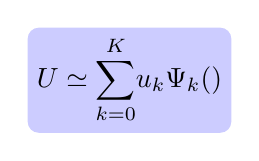
\begin{tikzpicture} \node [rounded corners,fill=blue!20] {
$U\simeq\displaystyle{\sum_{k=0}^{K}} u_k \Psi_k(\vxi)$
};
\end{tikzpicture}\hfill
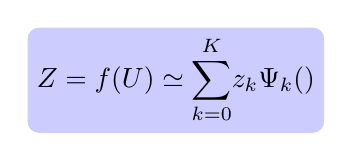
\begin{tikzpicture} \node [rounded corners,fill=blue!20] {
$Z=f(U)\simeq\displaystyle{\sum_{k=0}^{K}} z_k \Psi_k(\vxi)$
};
\end{tikzpicture}
\qquad
\qquad
}

\bi

\item For any model output of interest $f(X)$:
\bean
z_k = \frac{\langle Z \Psi_k \rangle}{\langle \Psi_k^2\rangle}= \frac{1}{||\Psi_k||^2} \int f(X(\vxi)) \, \Psi_k(\bm{\xi})
\pi_{\bm{\xi}}(\bm{\xi})d\bm{\xi}
\eean
\item Evaluate projection integral \textit{numerically}
\item Relies on black-box utilization of the computational model
\item Integral can be evaluated using
\bdi
\item A variety of (Quasi) Monte Carlo methods
\bi
\item Slow convergence; $\sim$ indep. of dimensionality
\ei
\item Quadrature/Sparse-Quadrature methods
\bi
\item Fast convergence; depends on dimensionality
\ei
\edi
\ei
\end{frame}


